\documentclass{beamer}

\beamertemplatenavigationsymbolsempty

\AtBeginSection[]
{
  \begin{frame}
    \tableofcontents[currentsection]
  \end{frame}
}

\title{Cryptography and You}
\author{Corey Ford, Liam Kirsh}
\institute{The White Hat}
\date{2015-01-14}

\begin{document}

\frame{\titlepage}

\section{Why Encrypt?}

\begin{frame}
  \frametitle{Why?}

Privacy and confidentiality

NSA?

\end{frame}

\section{Public-Key Encryption}

\begin{frame}
  \frametitle{Symmetric (Private-Key) Encryption}

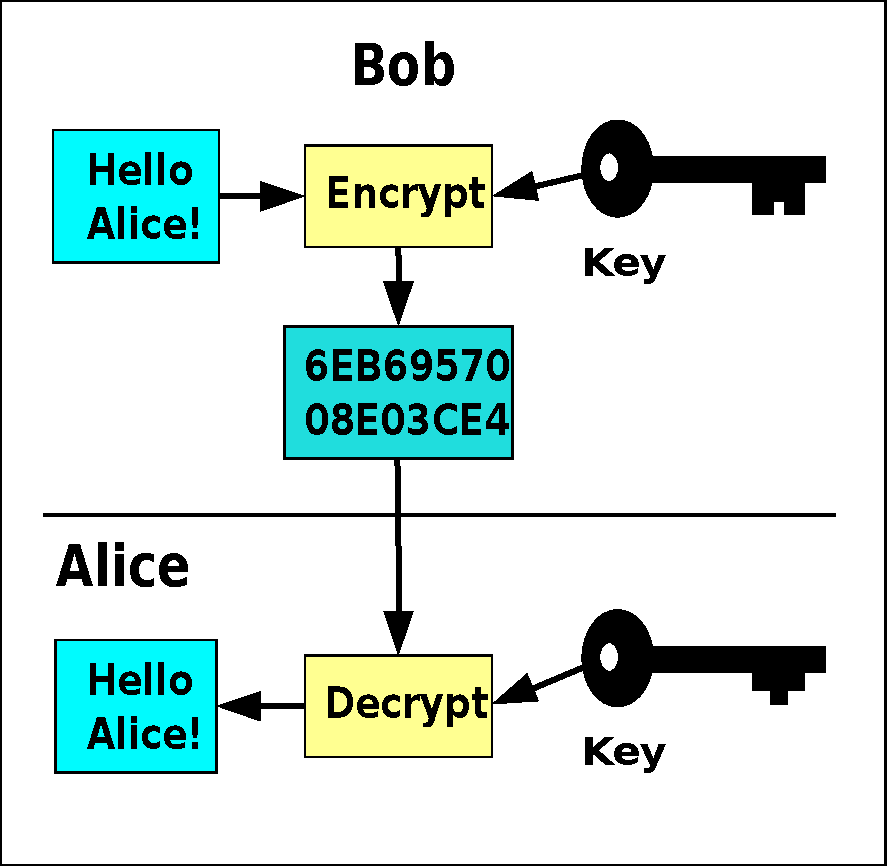
\includegraphics[height=0.5\textheight]{Symmetric_encryption}

\end{frame}

\begin{frame}
  \frametitle{Asymmetric (Public-Key) Cryptography}

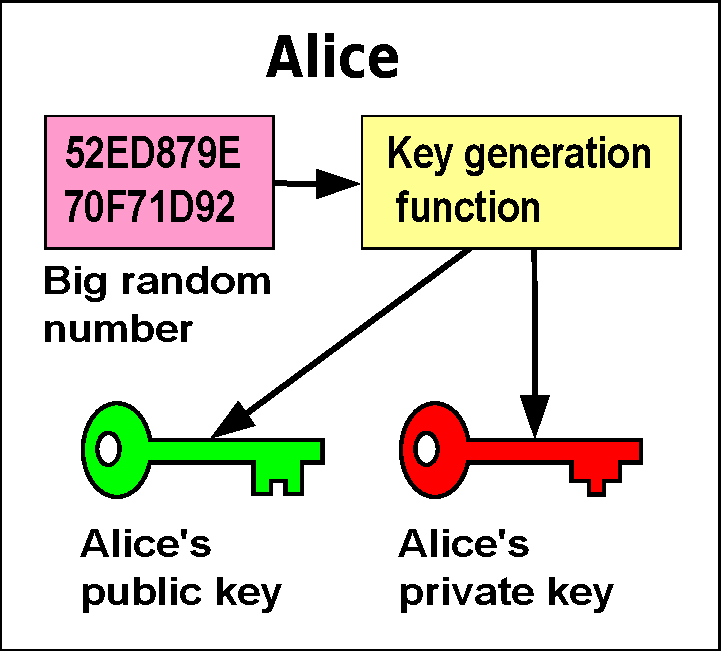
\includegraphics[height=0.5\textheight]{Public_key_making}

\end{frame}

\begin{frame}
  \frametitle{Asymmetric (Public-Key) Encryption}

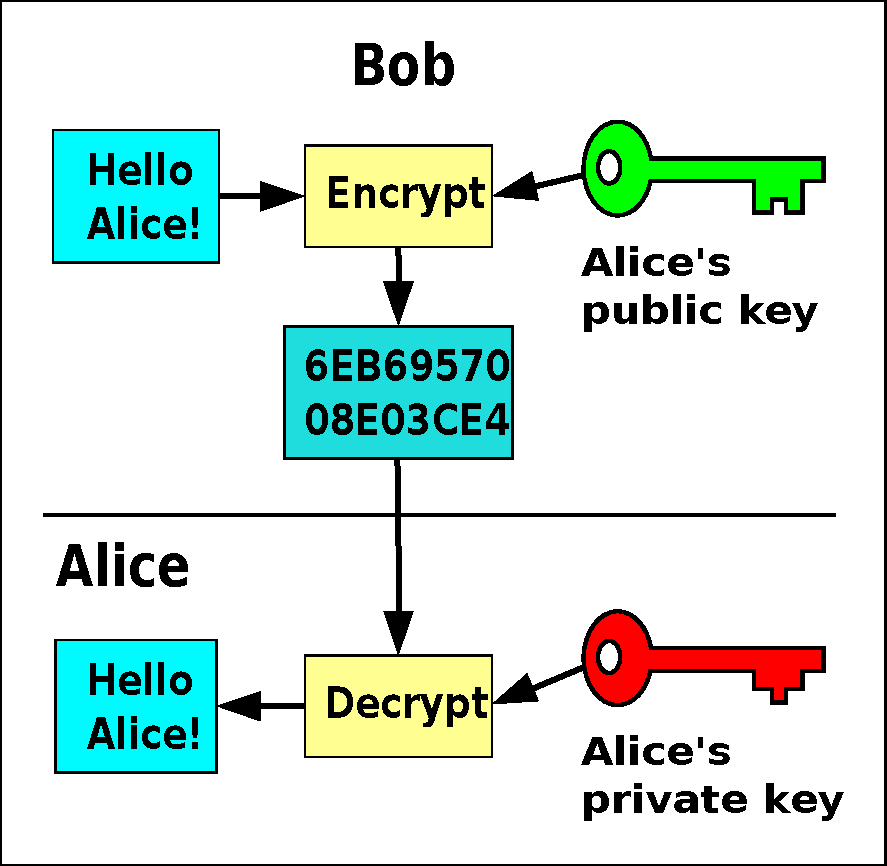
\includegraphics[height=0.5\textheight]{Public_key_encryption}

\end{frame}

\begin{frame}
  \frametitle{Asymmetric (Public-Key) Signatures}

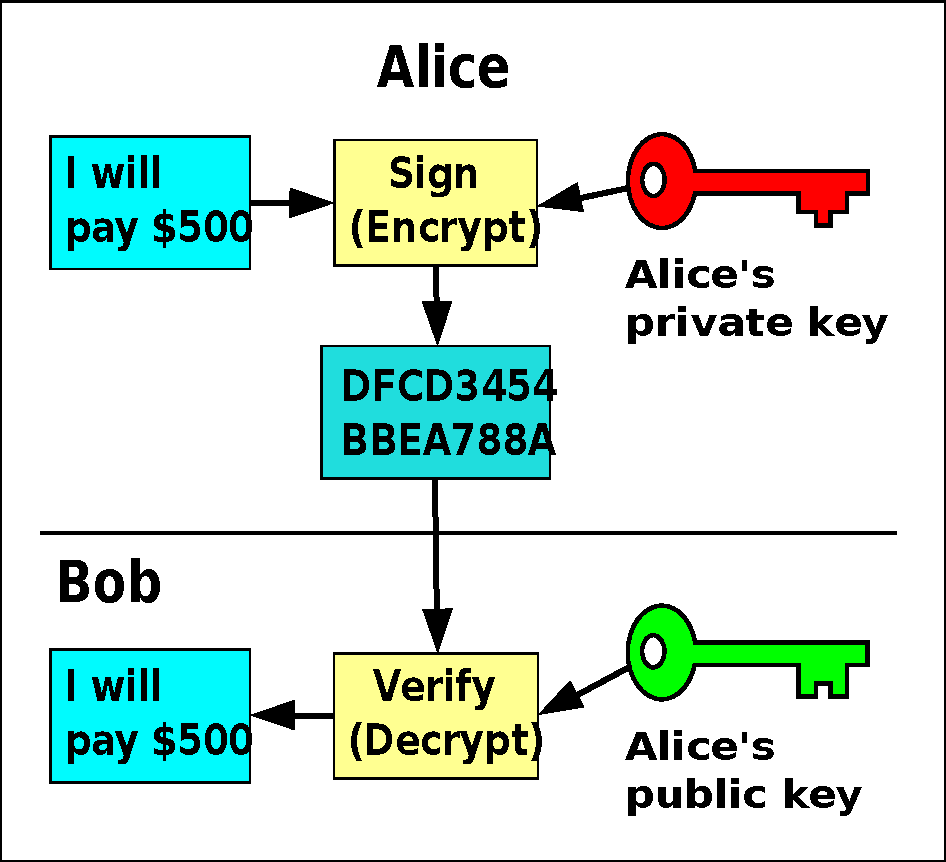
\includegraphics[height=0.5\textheight]{Public_key_signing}

\end{frame}

\begin{frame}
  \frametitle{RSA}

  \begin{itemize}
    \item finite group $\mathbb{Z}_N$ (modular arithmetic)
    \item choose large primes $p, q$, let $N = p \cdot q$
    \item $\phi(N) = (p - 1)(q - 1)$, with the property $$\forall_{x\in\mathbb{Z}_n}: x^{\phi(N)} = 1 \mod N$$
    \item choose $e, d$ such that $e \cdot d = 1 \mod \phi(N)$\\
    (hard to find $d$ given just $e$ and $N$)
  \end{itemize}
  \begin{align*}
  c &= [m^e \mod N]\\
  m &= [c^d \mod N]\\
    &= [(m^e)^d \mod N] = m
  \end{align*}
\end{frame}

\section{PGP}

\begin{frame}
  \frametitle{Pretty Good Privacy}

  \begin{itemize}
    \item encryption software for files, emails, \ldots
    \item public-key (RSA) encryption and signing
    \item ``keyring'' stores:
      \begin{itemize}
        \item public keys (lots)
        \item private keys (a few)
        \item user IDs (name, email)
        \item signatures on user IDs
        \item \ldots
      \end{itemize}
  \end{itemize}
\end{frame}

\begin{frame}
  \frametitle{History, Terminology}

  \begin{itemize}
    \item created by Phil Zimmerman in 1991
    \item circumvented export restrictions by publishing source code in a book
    \item OpenPGP: a standardized protocol
    \item GNU Privacy Guard (GnuPG): an open-source implementation
  \end{itemize}
\end{frame}

\begin{frame}
  \frametitle{Web of Trust}

  \begin{itemize}
    \item how to establish trust/identity?
    \item signatures on user IDs by other keys!
    \item decentralized (transitive) trust
    \item keyservers (untrusted) to distribute public keys
  \end{itemize}

  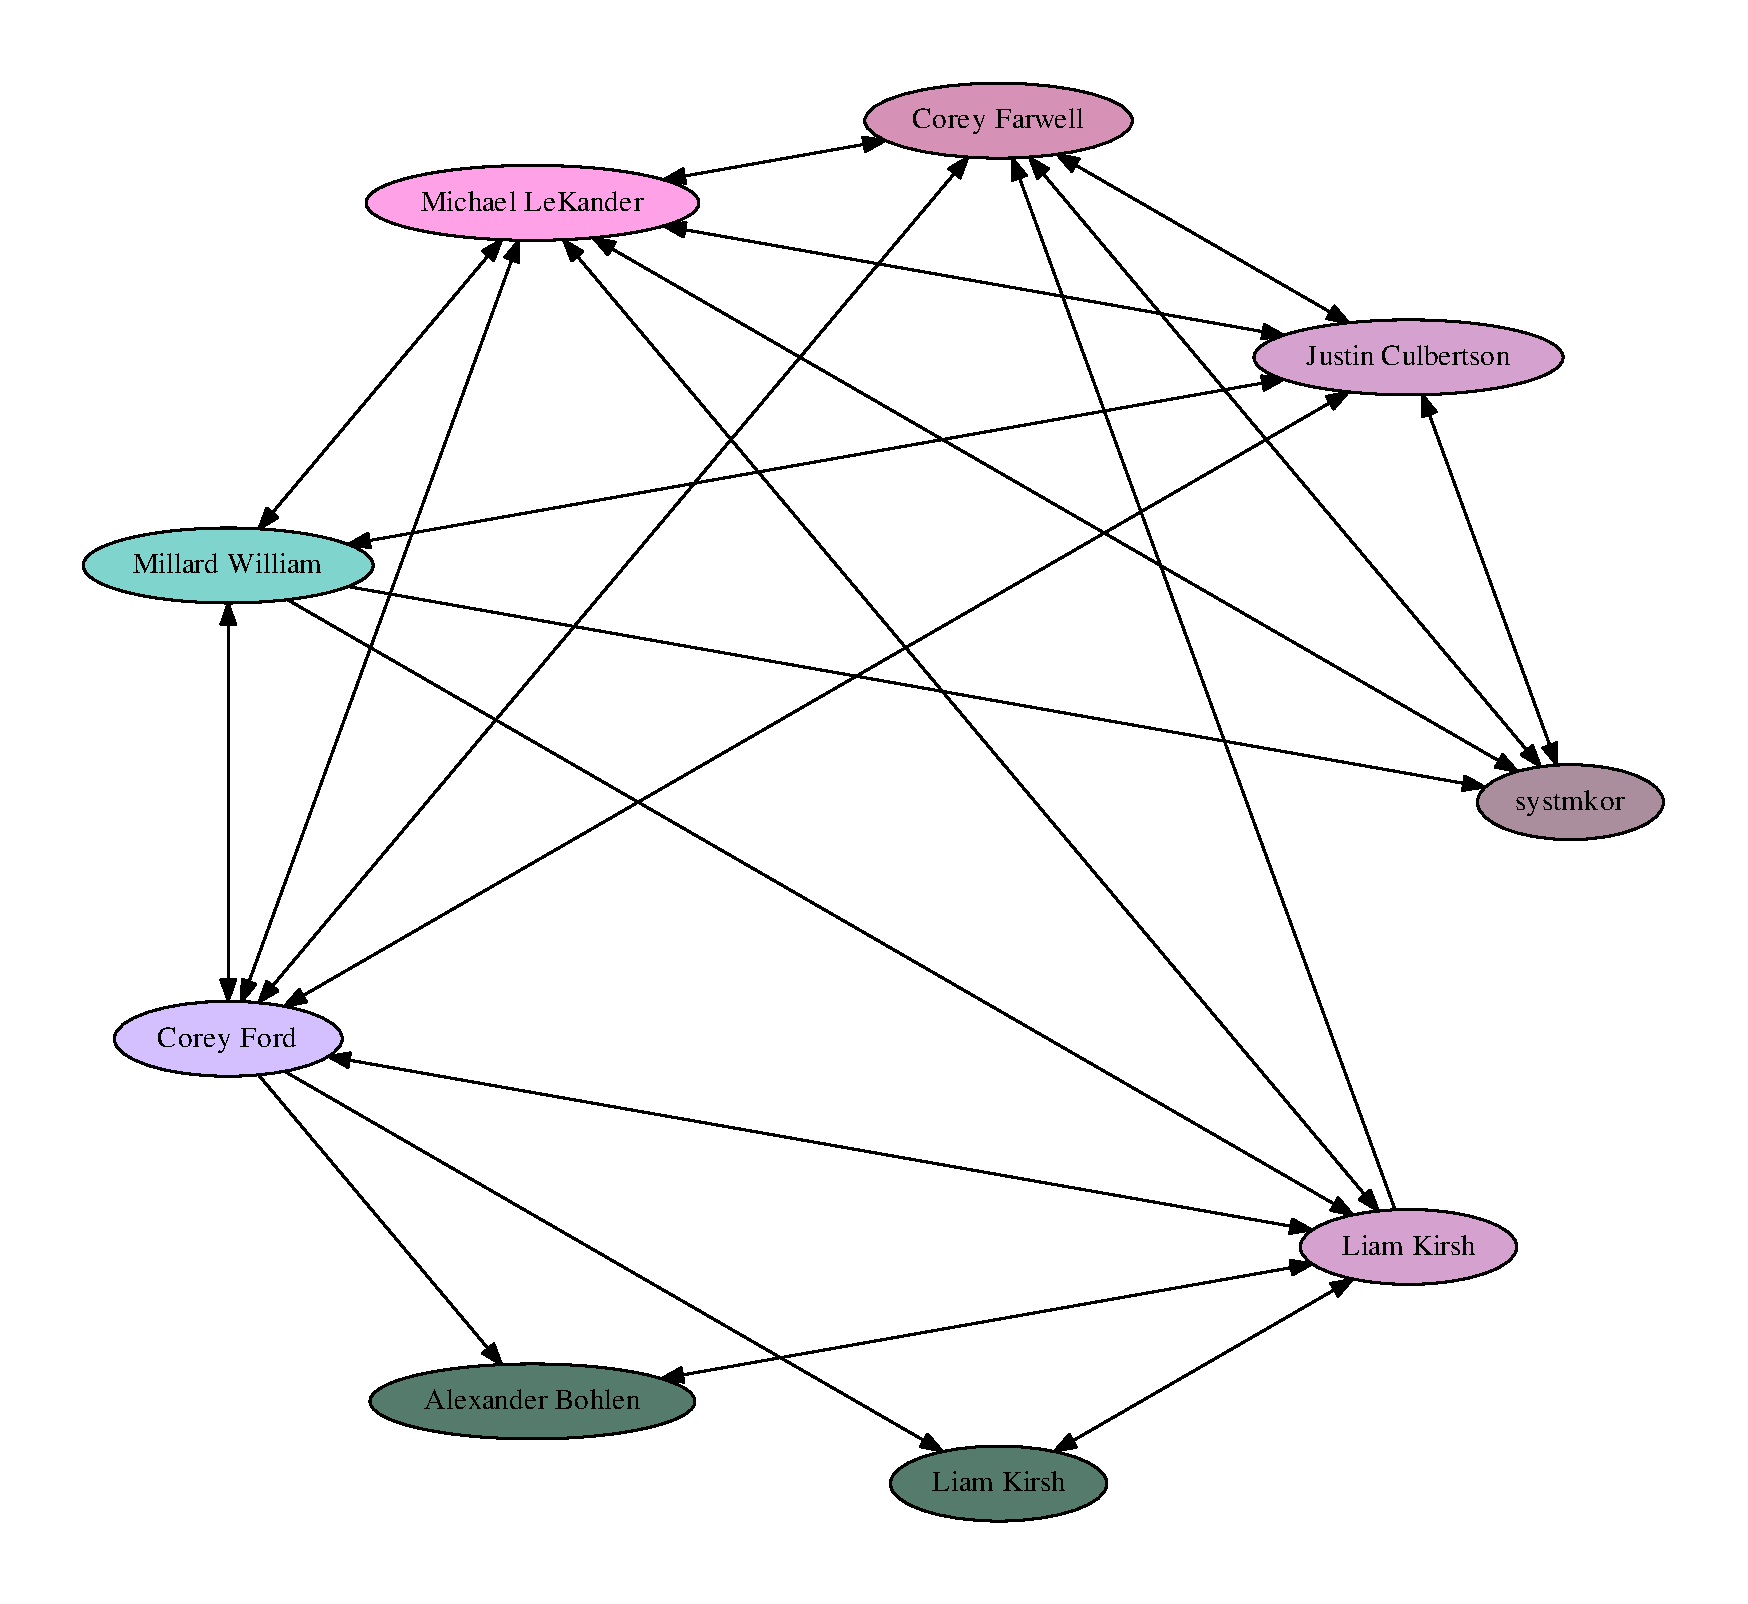
\includegraphics[height=0.5\textheight]{sigs}

\end{frame}

% \begin{frame}
%   \frametitle{Web of Trust}
%   \includegraphics[width=0.8\textwidth]{stats}
% \end{frame}

\section{Tutorial!}

\begin{frame}
  \frametitle{Do}

  \begin{enumerate}
    \item install stuff
      \begin{itemize}
        \item GnuPG (\url{gpgtools.org}, \url{gpg4win.org})
        \item Thunderbird + Enigmail (or use Apple Mail)
      \end{itemize}
    \item generate a key pair
    \item share public key (\url{pgp.mit.edu})
    \item sign keys
      \begin{itemize}
        \item find someone else who has uploaded their public key
        \item download it from a keyserver (by email or fingerprint)
        \item verify key fingerprint + identity (photo ID)
        \item if satisfied, sign key
        \item upload key again
      \end{itemize}
  \end{enumerate}

\end{frame}

\end{document}
